% !TeX program = lualatex

\documentclass[12pt]{report}
\usepackage[Glenn]{fncychap}
\usepackage[T1]{fontenc}
\usepackage[francais]{babel}
\usepackage{fontspec}
\usepackage{wrapfig}
\usepackage{graphicx}
\usepackage{subcaption}
\usepackage{caption}
\usepackage{soul}
\usepackage[colorlinks=true, linkcolor=black, urlcolor=black, citecolor=black]{hyperref}
% \usepackage[hyphens, spaces, obeyspaces]{url}
\usepackage[a4paper, width=175mm, top=25mm, bottom=25mm]{geometry}
\usepackage{parskip}
\usepackage{enumitem}
\usepackage{titlesec}
\usepackage{listings}
\usepackage{float}
\usepackage[final]{pdfpages}
\usepackage{xcolor}
\usepackage{tocbibind}
\usepackage{tocloft}
\usepackage{xpatch}
\usepackage{amsmath}
\usepackage{amsthm}
\usepackage{amsfonts}
\usepackage{graphics}
\usepackage{color}
% \usepackage[grey,utopia]{quotchap}
\usepackage{moreverb}
\usepackage{xcolor}
\usepackage{framed}
%\usepackage{arabluatex}
%\usepackage[algo2e, french, onelanguage, ruled]{algorithm2e}
\setlist[itemize]{label=\textbullet}
\usepackage{fancyhdr}
\pagestyle{fancy}   
\fancyhead{}
\fancyhead[C]{\leftmark}
\renewcommand{\headrulewidth}{0.4pt}
\renewcommand{\footrulewidth}{0.4pt}
\usepackage{xcolor}
\definecolor{light-gray}{gray}{0.90}
\usepackage{multirow}
\usepackage{soul}
\usepackage[utf8x]{inputenc}
\setcounter{secnumdepth}{3} 
\usepackage{dirtytalk}
\usepackage{csquotes}
\usepackage{mathtools}
\usepackage{amsmath}
\begin{document}
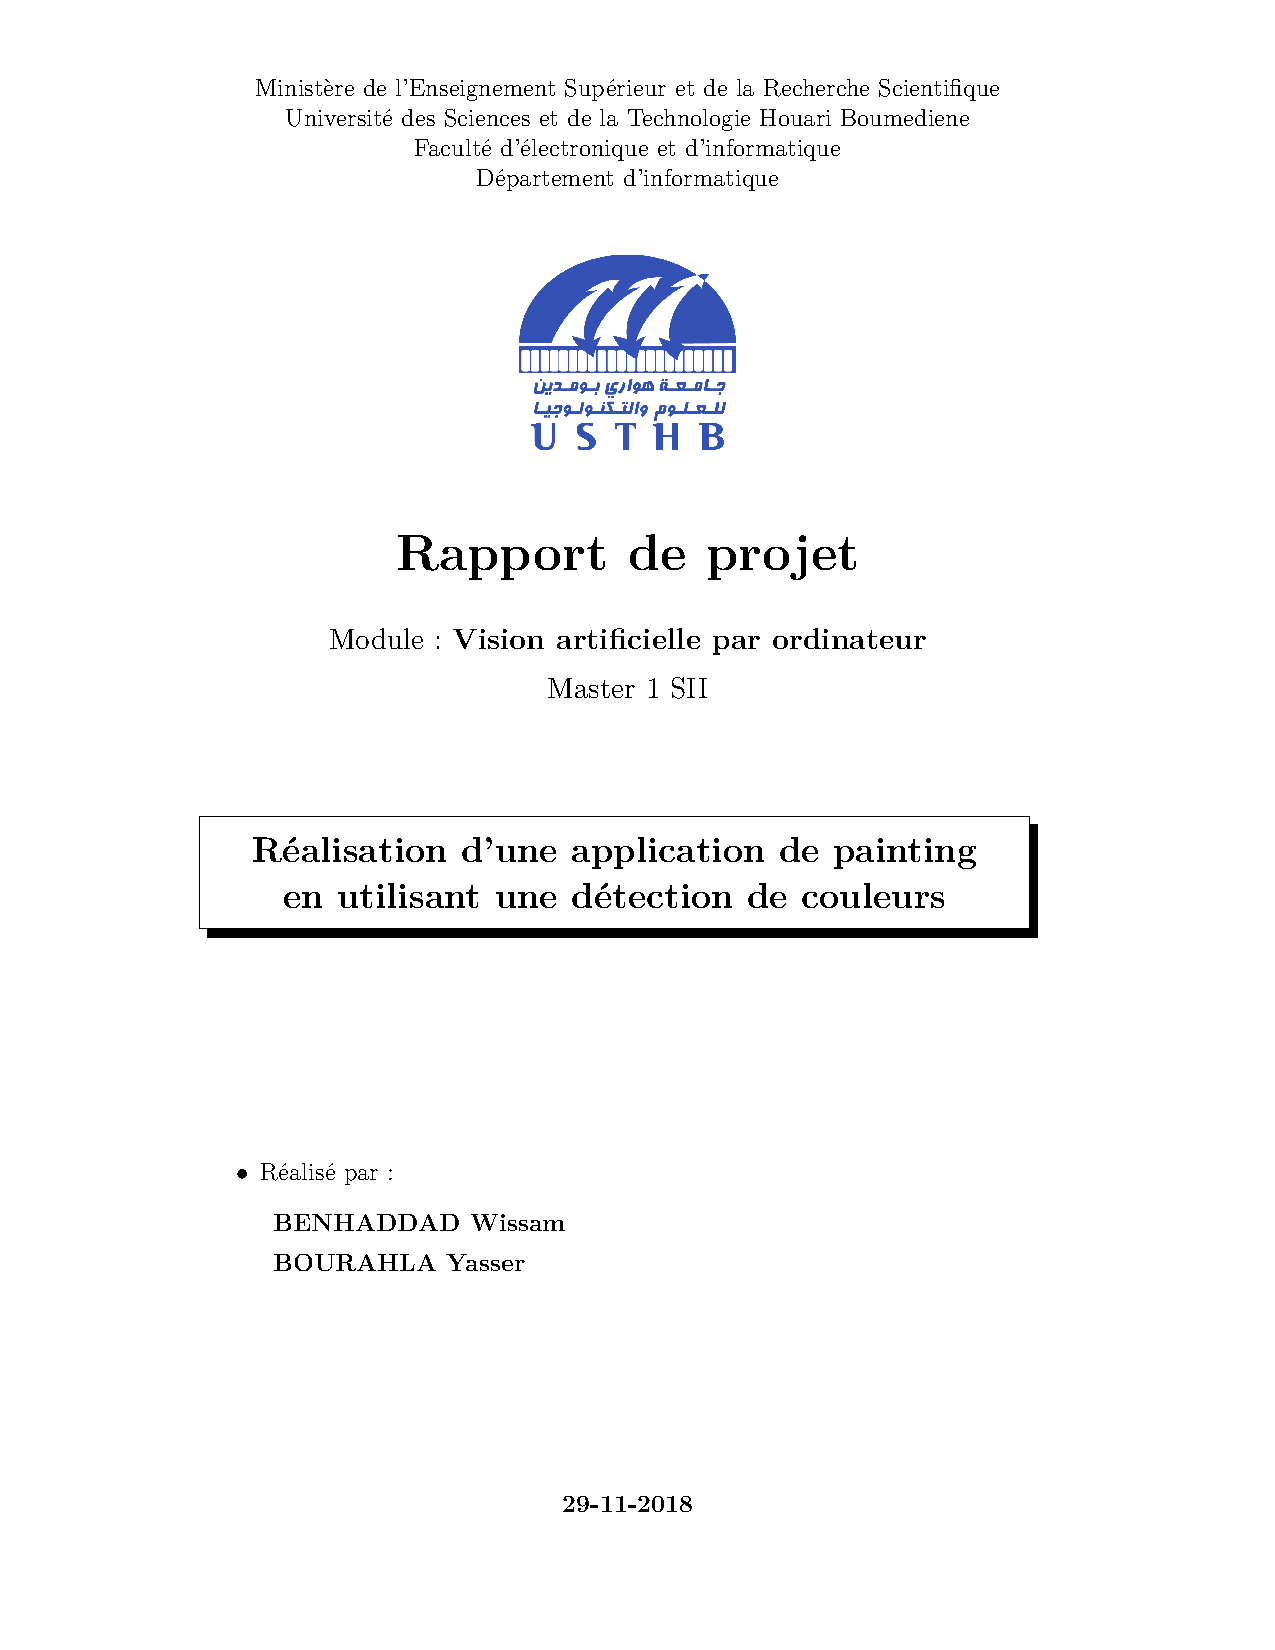
\includepdf[pages=1]{Page_garde.pdf} 
\tableofcontents
\listoffigures
\listoftables


\pagenumbering{arabic}
\newpage

\setlist[itemize]{label=\textbullet}
\chapter{Introduction}
	\section{Problématique et objectifs }
	\paragraph{}

\chapter{Solution proposées et implémentation}
Dans ce chapitre nous allons voir l'implémentation de l'algorithme lookAhead avec filtrage PC2 tel que décrit dans le chapitre précédent.
\section{Outils utilisés}
Pour l’implémentation de LookAhead nous avons opté à utiliser le langage de programmation C++ qui à la fois garde la rapidité du C tout en donnant la possibilité de modélisation orienté objet, et ceci en utilisant l'IDE de JetBrains CLion.
\begin{figure}[H]
	\centering
	\begin{subfigure}{.5\textwidth}
		\centering
		
\includegraphics[scale=0.3]{imgs/Clion.jpg}
		\label{fig:sub1}
	\end{subfigure}%
	\begin{subfigure}{.5\textwidth}
		\centering
		
\includegraphics[scale=0.08]{imgs/C++.png}
		\label{fig:sub2}
	\end{subfigure}
	\label{fig:test}
\end{figure}
\section{Implémentation}
Notre implémentation de LookAhead avec filtrage PC2 se compose de trois classes principales: Domains, Constraint et Solver.
\subsection{Domains}
Cette classe permet de gérer les domaines des variables, elle contient pour chaque variable son domaine initiale et son domaine courant, c’est à dire après application des algorithmes de filtrage ou instanciation de la variable. Les domaines sont représentés sous forme de listes d'entier.
\subsection{Constraint}
Chaque contrainte C(Xi,Xj) est représentée par une instance de cette classe, cette dernière contient une matrice nxm où n et m sont les tailles des domaines des variables Xi et Xj respectivement. Cette classe facilite les opérations sur les contraintes notamment la transposition, la composition et l’intersection.
\begin{figure}[H]
	\centering
	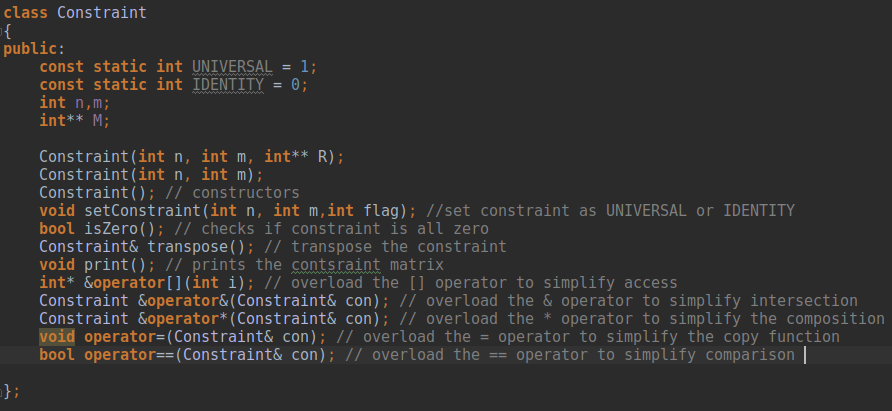
\includegraphics[scale=0.55]{imgs/constraint.png}
	\caption{L'espace de dessin}
	\label{fig:Cons}
\end{figure}
\subsection{Solver}
Un CSP est représenté par cette classe. Elle contient donc les paramètres composant un CSP <X,D,C>: les variables, leurs domaines ainsi que les contraintes entre eux. \\
Nous avons implémenté dans cette classe les algorithmes PC1, PC2 et lookAhead ainsi que la possibilité de choisir la variable à instancier en tirage aléatoire ou en suivant une heuristique.
\paragraph{LookAhead}
L’algorithme lookAhead a été implémenté comme décrit dans la figure \ref{fig:LookAhead}:
\begin{itemize}
\item On applique un filtre et on teste s’il y une inconsistance, sinon si toute les variables ont été instanciées.

\item On choisit la prochaine variable à instancier soit suivant une heuristique ou un ordre aléatoire.

\item On instancie la variable avec les valeurs possibles dans le domaine (qui a été mis à jour par le filtre).

\item On ajoute dans la queue le couple (i,i) pour le prochain appel de PC2.
\end{itemize}
\begin{figure}[H]
	\centering
	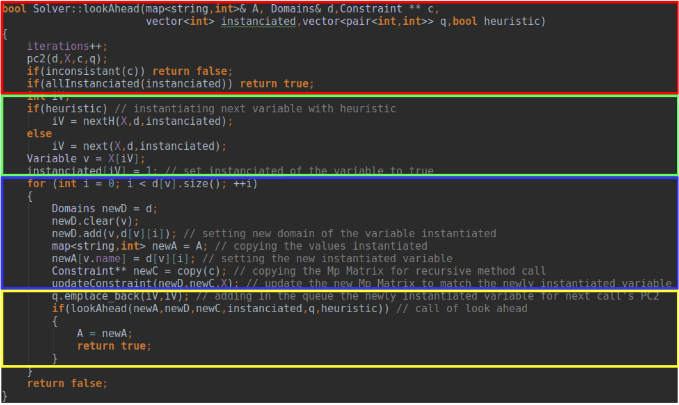
\includegraphics[scale=0.7]{imgs/lookA.png}
	\caption{L'algorithme lookAhead}
	\label{fig:LookAhead}
\end{figure}
\paragraph{Filtrage}
Nous avons implémenté les deux algorithmes de filtrage par chemin PC2 et PC1:
\begin{itemize}
	\item PC1 passe par toutes les variables à chaque fois et applique revise, si une entrée de la matrice Mp change, on refait la même chose.
	\begin{figure}[H]
		\centering
		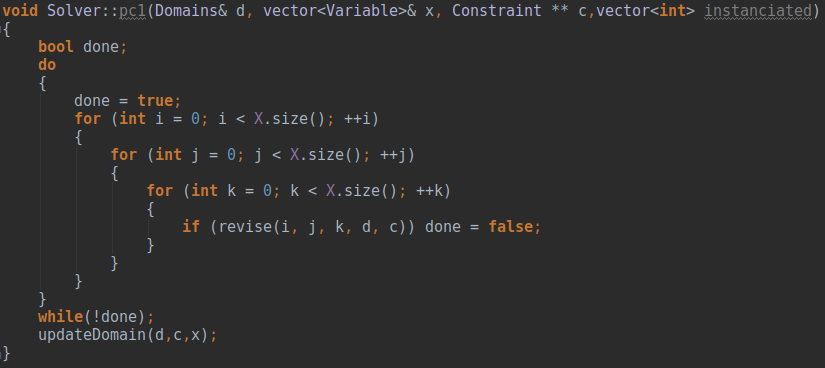
\includegraphics[scale=0.55]{imgs/pc1.png}
		\caption{L'algorithme PC1}
		\label{fig:PC1}
	\end{figure}
	\begin{figure}[H]
		\centering
		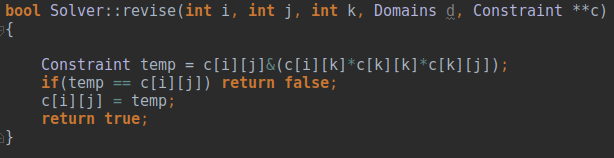
\includegraphics[scale=0.7]{imgs/revise.png}
		\caption{La fonction revise de PC1}
		\label{fig:Revise}
	\end{figure}
	\item PC2 quant à lui utilise une file pour garder les variables dont les entrées de la matrice Mp ont changé afin qu’il les traite.
	\begin{figure}[H]
		\centering
		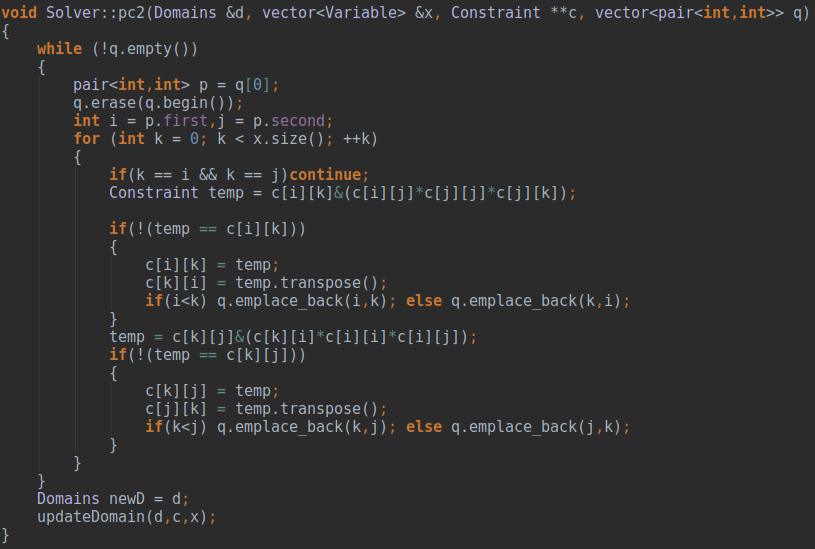
\includegraphics[scale=0.55]{imgs/pc2.png}
		\caption{L'algorithme PC2}
		\label{fig:PC2}
	\end{figure}
\end{itemize}
\paragraph{remarque:}
la fonction \textbf{updateDomain} mis à jour les domains de variables, dans les structures de listes cités avant dans ce chapitre.
\subsection{Génération aléatoire de CSP}
Afin de comparé les deux filtres PC1 et PC2 ainsi que le choix de variables aléatoire ou avec heuristique, nous avons implémenté une fonction qui génère un CSP aléatoire selon les paramètres suivant:
\begin{itemize}
	\item Nombre de variables: c’est le nombre de variables du CSP.
	
	\item Taille du domaine tailleD: la taille des domaines des variables varie entre tailleD*0,5 et tailleD*1,5 aléatoirement.
	
	\item Difficulté: ce paramètre représente la probabilité d’avoir un 0 dans la matrice d’une contrainte du CSP à générer. Plus ce paramètre est élevé, plus le CSP est difficile à satisfaire. 
\end{itemize}

\begin{figure}[H]
	\centering
	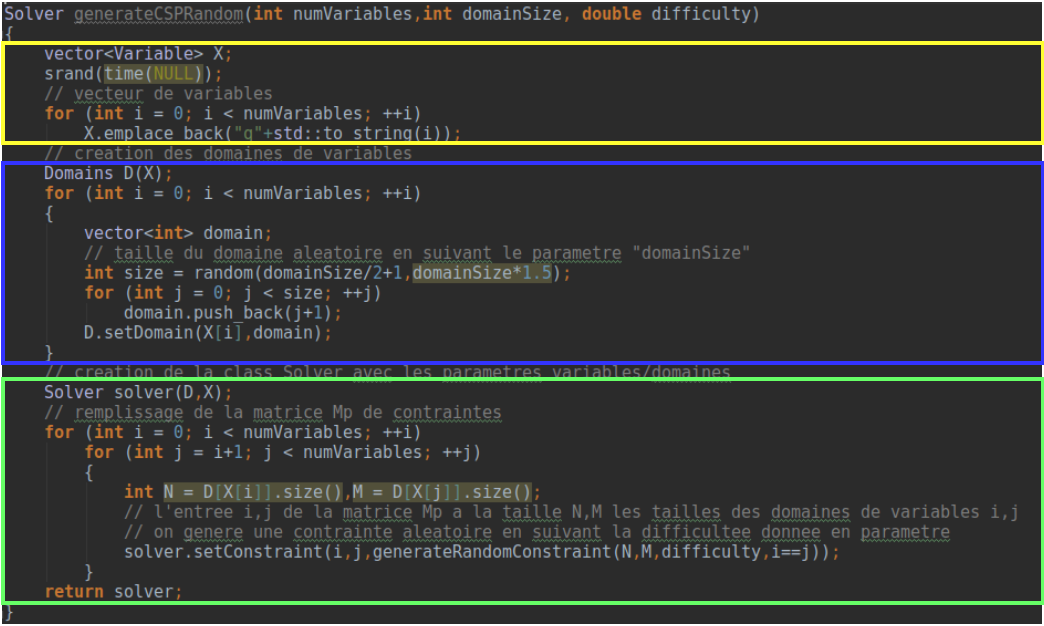
\includegraphics[scale=0.5]{imgs/random.png}
	\caption{L'algorithme PC2}
	\label{fig:Random}
\end{figure}

\section{Résultats}
Nous avons essayé l’algorithme lookAhead d’abord sur un problème connu, le problème des N-Reines. Ensuite nous avons généré des CSP aléatoirement avec des difficultés variables pour tester l’algorithme.
\subsection{N-Reines}
Pour tester les deux filtres PC1 et PC2 avec et sans heuristiques, nous avons généré le problème de N-Reines pour $N \in [4-14]$. les résultats sont résumé dans les figures suivantes:
\begin{figure}[H]
	\centering
	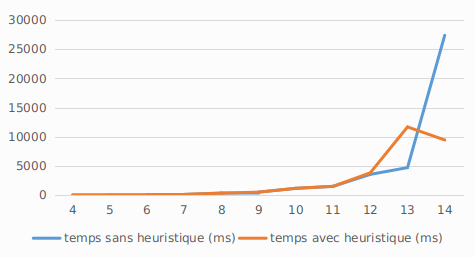
\includegraphics[scale=0.5]{imgs/queen1.png}
	\caption{Résultats de l'application de PC1 sur le problème des N-Reines }
	\label{fig:QueenPC1}
\end{figure}
\begin{figure}[H]
	\centering
	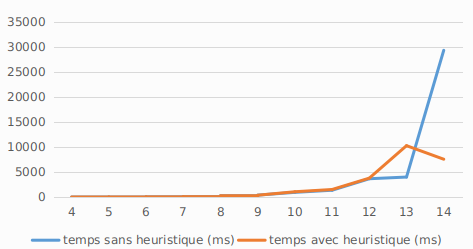
\includegraphics[scale=0.5]{imgs/queen2.png}
	\caption{Résultats de l'application de PC2 sur le problème des N-Reines}
	\label{fig:QueenPC2}
\end{figure}
\paragraph{}
On remarque que dans les deux cas l'heuristique ne donne pas toujours de meilleurs résultats. On remarque aussi que PC2 généralement surpasse PC1 comme le montre les tableaux suivants (les valeurs en rouge sont les valeurs ou PC1 a surpassé PC2):
\begin{figure}[H]
	\begin{tabular}{|c|c|c|c|c|c|c|c|c|c|c|c|}
		\hline
		
		nombre de reines&4&5&6&7&8&9&10&11&12&13&14 \\ \hline
		temps sans heuristique (ms)&2&8&48&85&269&382&937&1359&{\color{red}3659}&3999&{\color{red}29357}\\ \hline
		temps avec heuristique (ms)&3&8&35&71&258&362&1056&{\color{red}1507}&3779&10277&7567\\
		\hline
		
	\end{tabular}%
\caption{temps d'exécution de PC2 par nombre de reines}
\end{figure}
\begin{figure}[H]
	\begin{tabular}{|c|c|c|c|c|c|c|c|c|c|c|c|}
		\hline
		
		nombre de reines&4&5&6&7&8&9&10&11&12&13&14 \\ \hline
		temps sans heuristique (ms)&6&18&57&97&341&506&1143&1486&3542&4703&27391\\ \hline
		temps avec heuristique (ms)&5&17&62&112&317&493&1159&1492&3816&11680&9446\\
		\hline
		
	\end{tabular}%
	\caption{temps d'exécution de PC1 par nombre de reines}
\end{figure}

\subsection{Génération aléatoire de CSP}
Comme nous l’avons vu dans la partie précédente, l’algorithme de génération aléatoire de CSP dépend de trois valeurs: la difficulté, le nombre de variable et le domaine des variables. Dans cette partie nous allons voir comment la variation de un de ces paramètre affecte elle le temps d’exécution de l’algorithme lookAhead avec filtrage PC2.
\paragraph{Difficulté}
La difficulté représente la probabilité d’avoir un 0, donc si cette probabilité est très faible on arrive à satisfaire le CSP rapidement, même chose si elle est très élevé le filtrage PC2 trouve l’inconsistance rapidement. La figure suivante montre l'exécution de l'algorithme en prenant en paramètre le nombre de variable à 10 et le domaine qui varie de 9 à 27, la difficulté quant à elle est dans une échelle de 0 à 20 où la probabilité d’avoir 0 égale à 1 quand la difficulté est égale à 20.
\begin{figure}[H]
	\centering
	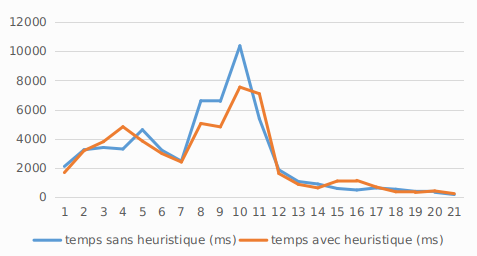
\includegraphics[scale=0.5]{imgs/random2.png}
	\caption{Variation de la difficulté en utilisant filtrage PC2}
	\label{fig:diff}
\end{figure}
\paragraph{Nombre de variables}
Plus on a un nombre de variable est grand, plus le temps de calcule augmente. Dans la figure suivante la difficulté a été fixée à 0,5 tandis que les tailles des domaines de variables varient entre 8 et 22.
\begin{figure}[H]
	\centering
	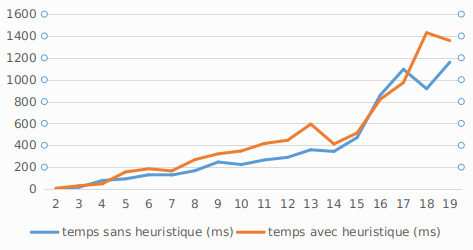
\includegraphics[scale=0.5]{imgs/variables.png}
	\caption{Variation du nombre de variables en utilisant filtrage PC2}
	\label{fig:vars}
\end{figure}
\paragraph{Taille du domaine}
La taille du domaine est elle aussi relié proportionnellement  au temps d’exécution. Dans la figure suivante la difficulté a été fixée à 0,5 tandis que le nombre de variables varient est à 8.
\begin{figure}[H]
	\centering
	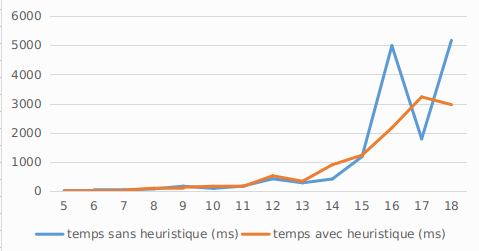
\includegraphics[scale=0.5]{imgs/domain.png}
	\caption{Variation des tailles des domaines en utilisant filtrage PC2}
	\label{fig:doms}
\end{figure}
\chapter{Conclusion générale}
\paragraph{}



\end{document}}

